\chapter{Implementation
    \label{chapter:implementation}}

This chapter discribs the tools, methods and reasons for the from of implementation.
As sad due to early test CLIP and TinyCLIP are used as models.

\section{Model acquisition}

The CLIP models are taken from the official CLIP Github repo \cite{clipgit}.
The TinyCLIP models are taken from the official TinyCLIP Github repo \cite{tinyclipgit}.
There is also the posibility to take models from HuggingFace \cite{huggingface}.
The problem with HuggingFace is that the model cant be split into image and text encoder.
Because of this reason only models from the offical CLIP repectiv TinyCLIP repo were used.

\section{Model translation}
The models were first split into image and text encoder.
The image encoder then gets translated to a onnx graph and afterwards simplified.
This onnx graph then is translated by the \acrshort{dfc} to \acrshort{har} and \acrshort{hef} files.

\begin{figure}
    \centering
    \subfloat[End of CLIP ResNet50x4 vision encoder Onnx graph acquired though official CLIP]{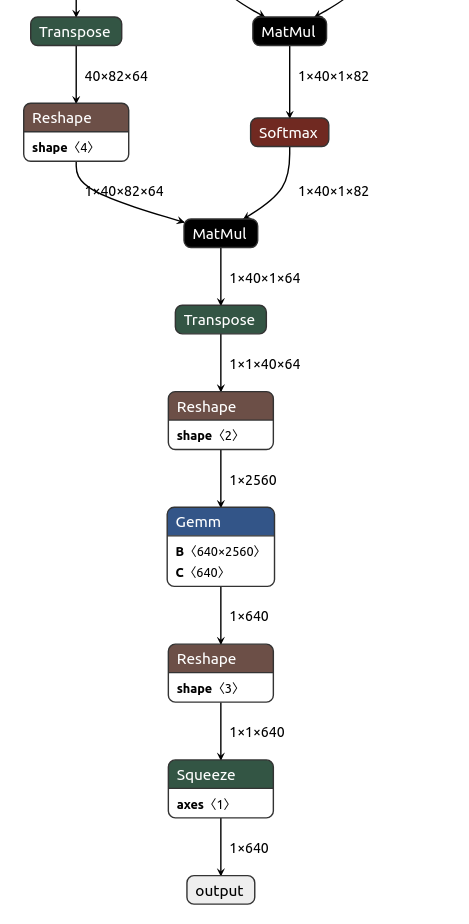
\includegraphics[width=0.4\textwidth]{Images/Implementation/ClipRes50x4.png}\label{fig:implementation:clipres50x4}}
    \qquad
    \subfloat[End of CLIP ResNet 50x4 vision encoder Onnx graph sendt by Hailo]{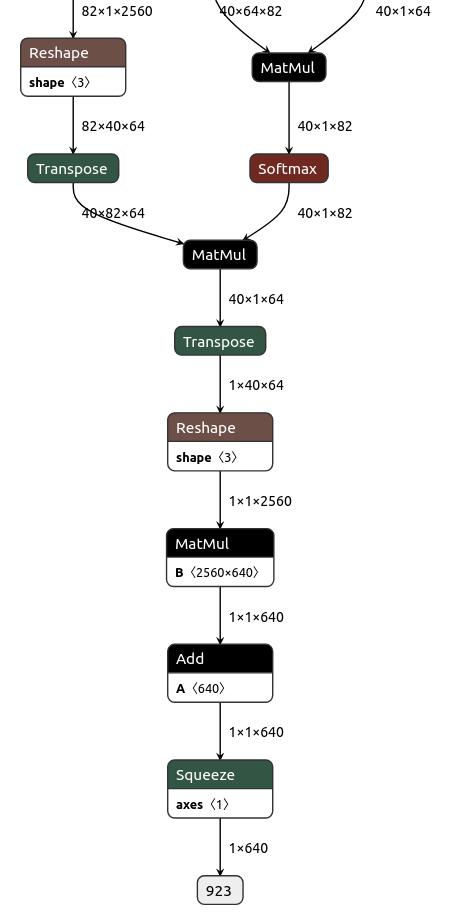
\includegraphics[width=0.4\textwidth]{Images/Implementation/HailoClipRes50x4.png}\label{fig:implementation:hailoclipres50x4}}
    \caption{Comparison of CLIP ResNet 50x4 vision encoder Onnx graph (a) from official CLIP and (b) from Hailo}
    \label{fig:implementation:compareRN50x4}
\end{figure}

In that step lays the first big problem of the project.
As described in \cref{section:dfc} the \acrshort{dfc} is unable to compile transformers.
To be precise, a transpose block at the end of every self attention layer is were the problems lay.
The \acrshort{dfc} swaps dimensions and takes together the last 2 dimensions.
In the ResNet which is acquired though the offical code (see \cref{fig:implementation:clipres50x4}) one can see that the transpose block after the MatMul block swaps a second and the third dimension.
This leads to a compilation error because the \acrshort{dfc} already combined the last 2 dimensions.
This error does not occure when the model given by Hailo is compiled.
In \cref{fig:implementation:hailoclipres50x4} the maximum of dimensions is 3.

To work around this problem the last part of the onnx graph is cut off.
To cut the graph Onnx-Modifier \cite{onnxmodifier} is used.
The cut off blocks are implemented as postprocessing.
As described in \cref{section:dfc} a script can be applied to change the behavior of the \acrshort{dfc}.
% Add scripts

After quantisation the graph can again be visualized with a tool name profiler from hailo.
In \cref{fig:implementation:compareRN50x4qunathar} the compiled model with the cutoff end is visualized.
In this figure the combination of the last dimensions can be seen.

\begin{figure}
    \centering
    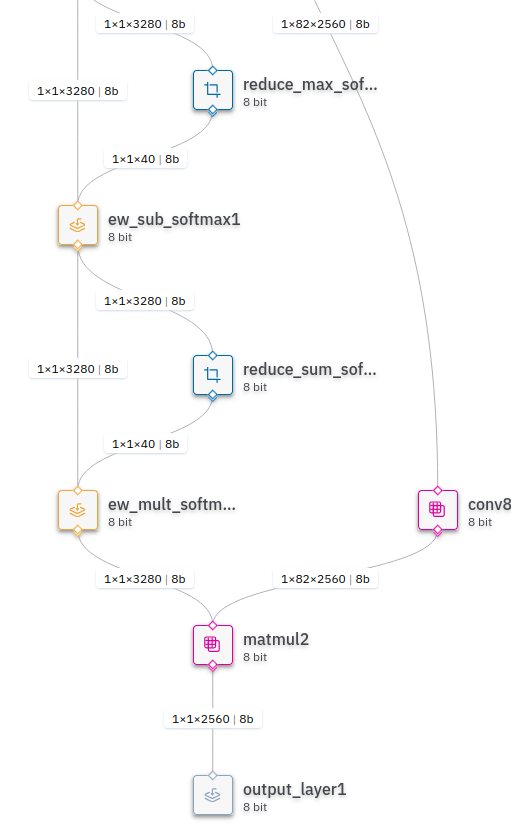
\includegraphics[width=0.4\textwidth]{Images/Implementation/ClipRes50x4_qunat_Har.png}
    \caption{Output of the \acrshort{dfc} from compiling the modified onnx graph of the ResNet50x4.}
    \label{fig:implementation:compareRN50x4qunathar}
\end{figure}

This graph then gets compiled to a \acrshort{hef} file which can be executed on Hailo hardware.
To use CLIP the text embeddings are also needed.
Due to the limitation that no transformers can be used with hailo the embeddings get calculated on a PC and the saved in a Json file.

\textbf{Comparison size}


\subsection{Preprocessing}

The hexagon dataset which is used as refrence consists of panorama pictures.
These pictuers get cut into 5 equal sized patches.
Every patch gets processed with CLIP.
To finally classify a image a mayority vote is taken over the subclasses of the patches.
This process is mentiond in Lia Winkler's report and increases the accuracy of the model.

\section{Inference}

To have a good comparison of performance the implementation on the Raspberry Pi is mostly similar to the one which is used on PC.
The PC application is mostly the same as Lia Winkler used in her work.
For Vision encoder only ResNet's were used because of the limitations from the \acrshort{dfc}.
The Hexagon dataset is used as image input.
As text input the subclasses from \cref{tab:dataset:subclasses} are used.
The text input were used solo or in a scentens.
In \cite{clip} the authors state that the performance of the network can improve if the text inputs are in a scentens.

To use the vision model on Hailo the python api is used.
2 diffrent implmentations were tested.
One proved much slower because the device initialisation happens every time a image is encoded.



\section{Measurments}